% PROSZĘ KOMPILOWAĆ TEN DOKUMENT ZA POMOCĄ SILNIKA XELATEX
% W PRZECIWNYM RAZIE NALEŻY USUNĄĆ PAKIET fontspec ORAZ USTAWIENIA FONTU
% Z PLIKU styles/prez_wmini_pl.sty (PIERWSZE TRZY LINIJKI)
% W PRZYPADKU BRAKU FONTU Adagio Slab NALEŻY ZGŁOSIĆ SIĘ DO BIP PW O JEGO UDOSTĘPNIENIE,
% ZAŁADOWAĆ INNY KRÓJ CZCIONKI LUB ZAKOMENTOWAĆ/USUNĄĆ USTAWIENIA FONTU

\documentclass[aspectratio=169]{beamer}

\usepackage{styles/prez_wmini_pl}
\usepackage{booktabs}
\setbeamertemplate{section in toc}[sections numbered]
\setbeamertemplate{subsection in toc}[subsections numbered]
\usepackage{times}
\usepackage{amsmath}
\usepackage{bm}

\usepackage{caption}
\captionsetup[figure]{labelformat=empty}

\usefonttheme[onlymath]{serif}

\definecolor{quotationcolour}{HTML}{F0F0F0}
\definecolor{quotationmarkcolour}{HTML}{1F3F81}

% Double-line for start and end of epigraph.
\newcommand{\epiline}{\hrule \vskip -.2em \hrule}
% Massively humongous opening quotation mark.
\newcommand{\hugequote}{%
  \fontsize{42}{48}\selectfont \color{quotationmarkcolour} \textbf{``}
  \vskip -.5em
}

% Beautify quotations.
\newcommand{\epigraph}[2]{%
  \bigskip
  \begin{center}
  \colorbox{quotationcolour}{%
    \parbox{.80\textwidth}{%
    \epiline \vskip 1em {\hugequote} \vskip -.5em
    \parindent 2.2em
    #1\vspace{-.25cm}\begin{flushright}\textsc{#2}\end{flushright}
    \epiline
    }
  }
  \end{center}
  \bigskip
}

\newcommand{\boldm}[1] {\mathversion{bold}#1\mathversion{normal}}

\graphicspath{ {./images/} }



% ------------------ Ustawienia użytkownika ------------------
% kolor tytułu prezentacji; zalecany white lub grafitowy.
% Poza tym można użyć zdefiniowanych w pakiecie kolorów:
% sloneczny, morelowy, mietowy, mokka, grafitowy, sliwkowy, szafirowy, wrzosowy
% lub wybrać sobie kolor z pakietu xcolor
\colorlet{title_color}{grafitowy}

\title{Opracowanie wirtualnego środowiska\\do symulacji dynamiki lotu\\ bezzałogowych statków powietrznych}
%\subtitle{Podtytuł consectetur adispiscing elit}
\author{Wojciech Gajda \and  Igor Faliszewski}
\date{7 luty 2024} % można tam wpisać datę jaką się chce lub zakomentować dla daty dzisiejszej



% ------------------ Początek prezentacji ------------------

\begin{document}
\sloppy

% Slajd tytułowy WG
{
\maketitleframe 
}

\begin{frame}
\frametitle{Agenda}
  \tableofcontents[  
    sectionstyle=show, 
    %hideallsubsections
    ]
\end{frame}


\section{Wstep}

\begin{frame}%[allowframebreaks]
	\frametitle{O projekcie}
	\begin{columns}
		\begin{column}{0.33\textwidth}
	   	 	\begin{figure}
	   		 \centering
	      		 \uncover<2->{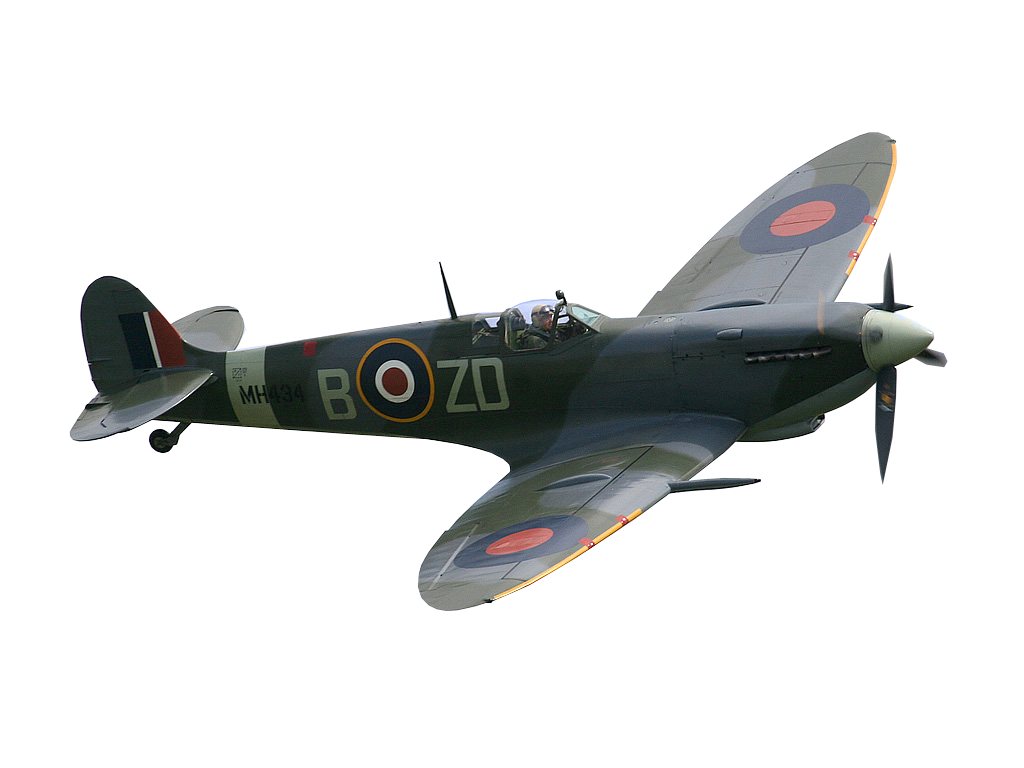
\includegraphics[width=0.9\textwidth]{spitfire.png}}
	    		\end{figure}
		\end{column}
		\begin{column}{0.33\textwidth}
	   	 	\begin{figure}
	   		 \centering
	      		 \uncover<3->{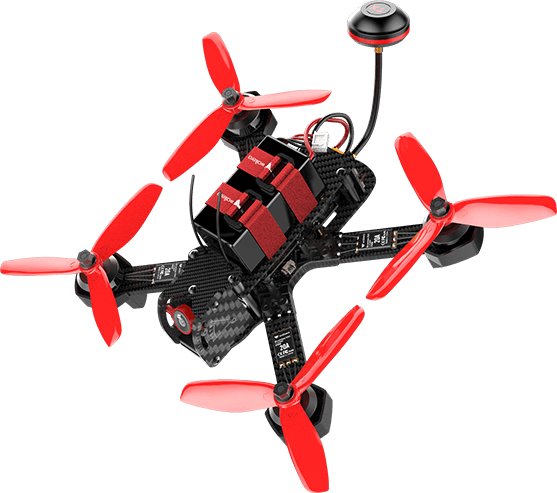
\includegraphics[width=0.9\textwidth]{quadcopter_fpv.png}}
	    		\end{figure}
		\end{column}
		\begin{column}{0.33\textwidth}
	    		\begin{figure}
	   		 \centering
	      		 \uncover<4->{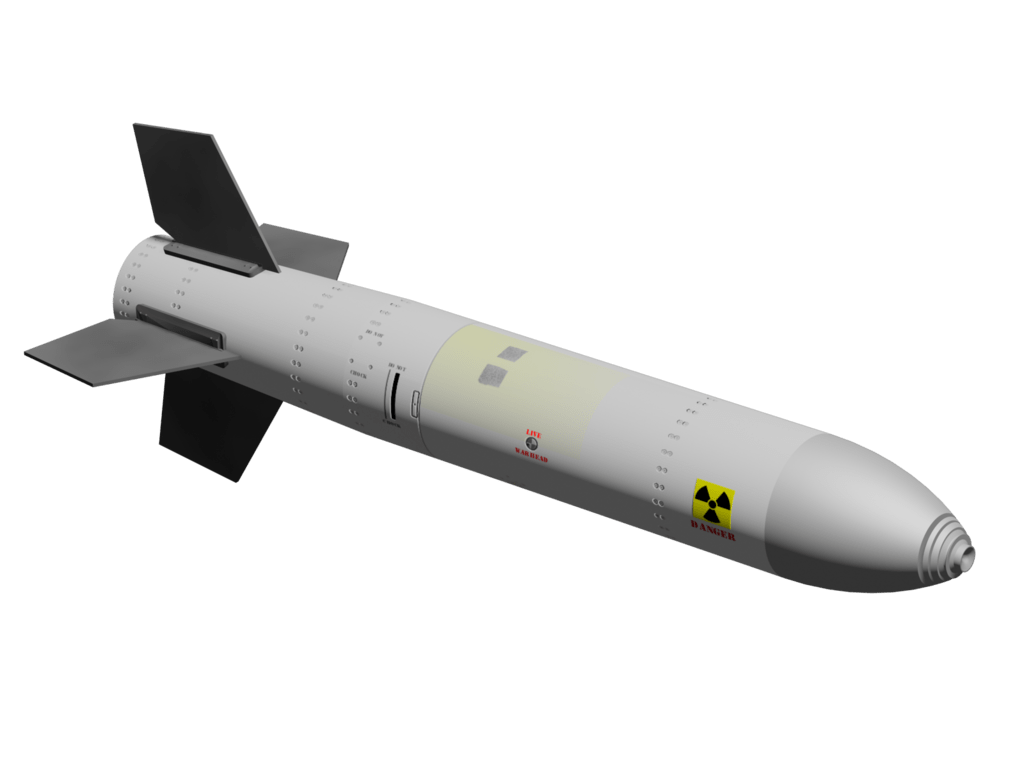
\includegraphics[width=0.9\textwidth]{missile.png}}
	    		\end{figure}
		\end{column}
	\end{columns}
\end{frame}

\begin{frame}%[allowframebreaks]
	\frametitle{Cel projektu}
	  \begin{itemize}
	  \item<2->{
	    Kompleksowa symulacja fizyki.
	  }
	  \item<3-> {   
	    Wysoka konfigurowalność BSP, środowiska i symulacji.
	  }
	  % Można ustalić kiedy dany element ma się pojawić, używając <n->:
	  \item<4-> {
	    Bogate narzędzie dla analityków i developerów.
	  }
	  \item<5-> {
	    Licencja open-source.
	  }
 	 \end{itemize}
\end{frame}

\begin{frame}%[allowframebreaks]
	\frametitle{Wstep teoretyczny I}
	 \uncover<2->{\epigraph{There is nothing so practical as a good theory.}{Lewin Kurt}}
	 \uncover<3->{\epigraph{Nie ma osobnej ani teorii, ani praktyki inżynierskiej, jest tylko wspólna sztuka inżynierska.}{prof. Jan Oderfeld}}
\end{frame}

\begin{frame}%[allowframebreaks]
	\frametitle{Wstep teoretyczny II}
	Tematyka poruszona we wstępie teoretycznym:
	\begin{itemize}
	  \item<2->{
	    dynamika lotu BSP,
	  }
	  \item<3-> {   
	    sterowania i nawigacja BSP,
	  }
	  \item<4-> {
	    grafika komputerowa 3D,
	  }
	  \item<5-> {
	    graficzny interfejs użytkownika,
	  }
	  \item<6->{
	    udźwiękowienie.
	  }
 	 \end{itemize}
\end{frame}




\section{Specyfikacja}

\begin{frame}
	\frametitle{Wymagania funkcjonalne}
	\begin{columns}[T]
	  \begin{column}{.33\textwidth}
	  \uncover<2->{
	    \begin{figure}
	      
\includegraphics[width=0.95\textwidth]{pilot.png}
	      %\caption{Użytkownik -- operator}
	    \end{figure}
	    }
	  \end{column}
	
	  \begin{column}{.33\textwidth}
	  \uncover<3->{
	    \begin{figure}
	      
\includegraphics[width=\textwidth]{scientist.jpg}
	      %\caption{Analityk}
	    \end{figure}
	    }
	  \end{column}
	
	  \begin{column}{.33\textwidth}
	  \uncover<4->{
	    \begin{figure}
	      
\includegraphics[width=0.9\textwidth]{dev.png}
	      %\caption{Developer}
	    \end{figure}
	    }
	  \end{column}
	\end{columns}
	
	\vspace{8pt}
	
	\begin{columns}[T]
	  \begin{column}{.33\textwidth}
	   \centering
	   \uncover<2->{Użytkownik -- operator}
	  \end{column}
	
	  \begin{column}{.33\textwidth}
	  \centering
	      \uncover<3->{Analityk}
	  \end{column}
	
	  \begin{column}{.33\textwidth}
	   \centering
	  \uncover<4->{Developer}
	  \end{column}
	\end{columns}
\end{frame}

\begin{frame} % IF
    \frametitle{Dobór technologii} % loga róznorakie
    
    \begin{columns}
        \begin{column}{0.33\textwidth}
            \begin{figure}
                \centering
                \uncover<2->{
\includegraphics[height=0.2\textheight]{logos/cpp.png}}
            \end{figure}
            \begin{figure}
            \centering
            \uncover<5->{
\includegraphics[height=0.2\textheight]{logos/eigen.png}}
            \end{figure}
        \end{column}
        \begin{column}{0.33\textwidth}
            \begin{figure}
                \centering
                \uncover<3->{
\includegraphics[height=0.2\textheight]{logos/java.png}}
            \end{figure}
            \begin{figure}
                \centering
                \uncover<6->{
\includegraphics[height=0.2\textheight]{logos/zmq.png}}
            \end{figure}
        \end{column}
        \begin{column}{0.33\textwidth}
            \begin{figure}
                \centering
                \uncover<4->{
\includegraphics[height=0.2\textheight]{logos/rust.png}}
            \end{figure}
            \begin{figure}
                \centering
                \uncover<7->{
\includegraphics[height=0.2\textheight]{logos/opengl.png}}
            \end{figure}
        \end{column}
    \end{columns}
\end{frame}

\begin{frame} % WG
	\frametitle{Architektura I}
	\begin{itemize}
		\item<2-> UAV\_visualization
		\item<3-> UAV\_physic\_engine
		\item<4-> UAV\_controller
		\item<5-> UAV\_drop\_physic
		\item<6-> UAV\_aggregator
		\item<7-> UAV\_common
		\item<8-> UAV\_server
		\item<9-> UAV\_map\_generator
	\end{itemize}
\end{frame}

\begin{frame}
	\frametitle{Architektura II}
	\begin{figure}
		\centering
		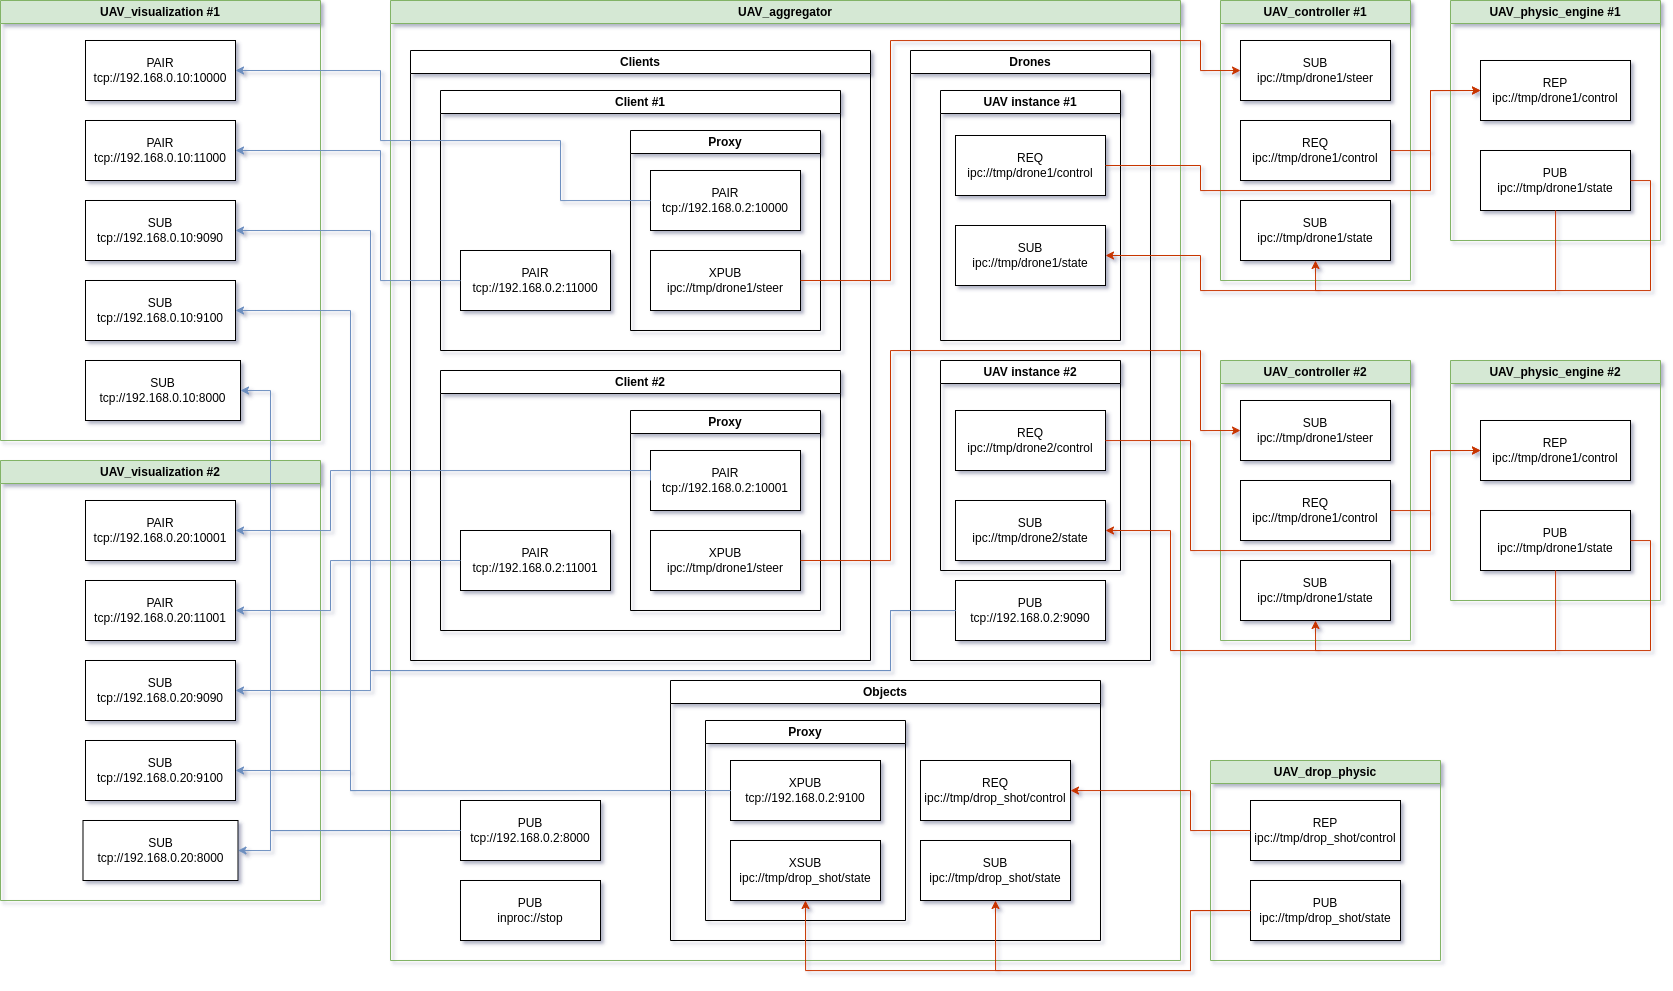
\includegraphics[width=0.8\textwidth]{ZMQinMINIUAV.drawio.png}
	\end{figure}
\end{frame}

\section{Demonstracja}

\begin{frame}
	  \begin{center}
	\Huge Demo
	\end{center}
\end{frame}

\begin{frame}
	\frametitle{Dyskusja}
	\begin{figure}
		\centering
		
\includegraphics[width=0.7\textwidth]{questions.png}
	\end{figure}
\end{frame}


\begin{frame}
	  \begin{center}
	\Huge Dziękujemy za uwagę!
	\end{center}
\end{frame}

\end{document}